\documentclass{standalone}
\usepackage{pgfplots}
\pgfplotsset{compat=1.18}
\usepgfplotslibrary{colorbrewer}
\pgfplotsset{cycle list/Set1-6}

\begin{document}

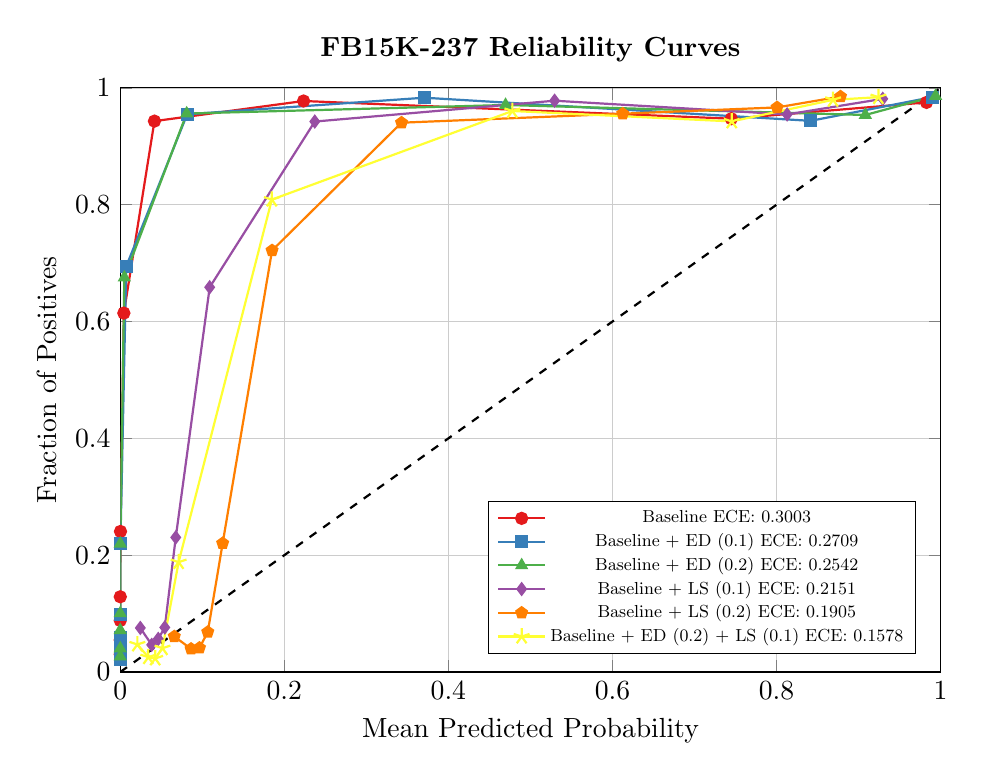
\begin{tikzpicture}
\begin{axis}[
    title={\textbf{FB15K-237 Reliability Curves}},
    xlabel={Mean Predicted Probability},
    ylabel={Fraction of Positives},
    xmin=0, xmax=1,
    ymin=0, ymax=1,
    xtick={0, 0.2, 0.4, 0.6, 0.8, 1.0},
    ytick={0, 0.2, 0.4, 0.6, 0.8, 1.0},
    legend pos=south east,
    legend style={nodes={scale=0.7, transform shape}, font=\small},
    grid=both,
    grid style={line width=.1pt, draw=gray!20},
    major grid style={line width=.2pt, draw=gray!40},
    width=12cm,
    height=9cm,
    cycle list name=Set1-6
]

% Perfectly Calibrated Line
\addplot [color=black, dashed, line width=0.8pt, forget plot]
    coordinates {(0,0)(1,1)};

% Model 1: Baseline
% File: fb15k237_baseline.txt 
\addplot+[mark=*, thick] coordinates {
    (7.64247138e-09, 0.03028823) (3.73450050e-07, 0.05472758) (4.57216904e-06, 0.08817782) (3.61842894e-05, 0.12878788)
    (2.85698287e-04, 0.24065478) (4.37984329e-03, 0.61446372) (4.16690817e-02, 0.94307354) (2.23452529e-01, 0.9775226)
    (7.44872033e-01, 0.94722697) (9.82812427e-01, 0.97508549)
};
\addlegendentry{Baseline ECE: 0.3003}

% Model 2: Baseline + ED (0.1)
% File: fb15k237_ed_0.1.txt 
\addplot+[mark=square*, thick] coordinates {
    (7.06140139e-10, 0.02149487) (6.42192567e-08, 0.04129001) (1.14475827e-06, 0.05912534) (1.28397724e-05, 0.09821647)
    (1.74048029e-04, 0.21988761) (7.31288472e-03, 0.69435622) (8.15617739e-02, 0.95480088) (3.70683115e-01, 0.98314195)
    (8.41528478e-01, 0.94356218) (9.89791149e-01, 0.98412311)
};
\addlegendentry{Baseline + ED (0.1) ECE: 0.2709}

% Model 3: Baseline + ED (0.2)
% File: fb15k237_ed_0.2.txt 
\addplot+[mark=triangle*, thick] coordinates {
    (3.10811739e-11, 0.02638007) (7.63909715e-09, 0.04031273) (2.53771226e-07, 0.07158563) (4.31989170e-06, 0.10041534)
    (8.08379661e-05, 0.21964329) (4.95505135e-03, 0.67529929) (8.09656606e-02, 0.95602248) (4.69685332e-01, 0.97068165)
    (9.08257778e-01, 0.95357928) (9.93836925e-01, 0.98607719)
};
\addlegendentry{Baseline + ED (0.2) ECE: 0.2542}

% Model 4: Baseline + LS (0.1)
% File: fb15k237_ls_0.1.txt 
\addplot+[mark=diamond*, thick] coordinates {
    (0.02446789, 0.07547631) (0.0383413, 0.04642072) (0.04630501, 0.05668214) (0.05427448, 0.07622771)
    (0.06764979, 0.23039335) (0.10904234, 0.65868556) (0.23714154, 0.94234058) (0.52944681, 0.97801124)
    (0.8129288, 0.95455656) (0.92947417, 0.98119199)
};
\addlegendentry{Baseline + LS (0.1) ECE: 0.2151}

% Model 5: Baseline + LS (0.2)
% File: fb15k237_ls_0.2.txt 
\addplot+[mark=pentagon*, thick] coordinates {
    (0.06587381, 0.06082071) (0.08633259, 0.03957977) (0.09653018, 0.04129001) (0.10668505, 0.06840948)
    (0.12483557, 0.22037625) (0.1850612, 0.72172001) (0.34289518, 0.94038602) (0.61249397, 0.95577816)
    (0.80064556, 0.96652822) (0.87798829, 0.98510015)
};
\addlegendentry{Baseline + LS (0.2) ECE: 0.1905}

% Model 6: Baseline + ED (0.2) + LS (0.1)
% File: fb15k237_combined.txt 
\addplot+[mark=star, thick, mark size=3pt] coordinates {
    (0.0208823, 0.04714216) (0.0342311, 0.02540924) (0.04257162, 0.02321036) (0.05146143, 0.04080137)
    (0.07114375, 0.18812607) (0.18478309, 0.80869778) (0.47797199, 0.96042023) (0.74544392, 0.9425849)
    (0.86888412, 0.97947716) (0.92417137, 0.98412311)
};
\addlegendentry{Baseline + ED (0.2) + LS (0.1) ECE: 0.1578}

\end{axis}
\end{tikzpicture}

\end{document}